% http://tex.stackexchange.com/questions/11866/compile-a-latex-document-into-a-png-image-thats-as-short-as-possible#11880
%http://tex.stackexchange.com/questions/152247/best-practice-to-include-standalone-precompiled-graphics
\documentclass[border=1pt]{standalone}
\usepackage{tikz}

\begin{document}

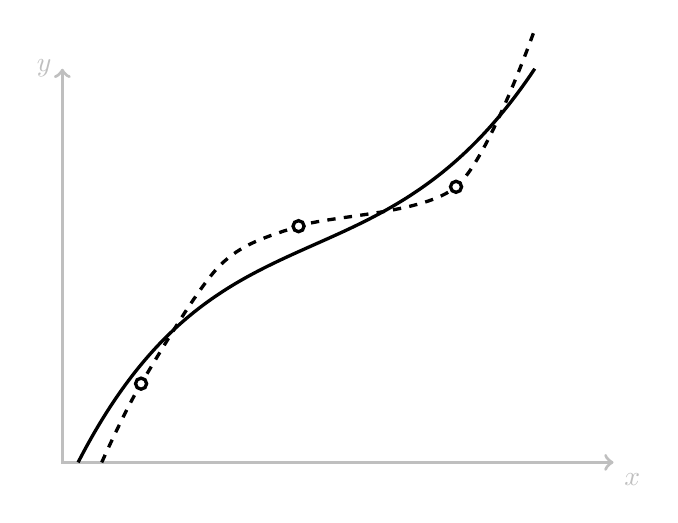
\begin{tikzpicture}[very thick]
	%\coordinate (A1) at (0,0);
	%\coordinate (A2) at (6, 4);
	%\draw [help lines, lightgray] (A1) grid (A2);
	\draw [<->, lightgray] (0,5) node[left] {$y$} -- (0, 0) -- (7, 0) node[below right] {$x$};

	\newcommand*{\ps}{2pt} % point size

	\draw[dashed] plot [smooth] coordinates {(0.5,0) (1,1) (2,2.5) (3,3) (5,3.5) (6,5.5)};
	\draw[fill=white] (1,1) circle (\ps);
	\draw[fill=white] (3,3) circle (\ps);
	\draw[fill=white] (5,3.5) circle (\ps);
	%\draw (0.5, 1) -- (6,4.5);
	\draw (0.2,0) .. controls (2,3.5) and (4,2) .. (6,5);

\end{tikzpicture}

\end{document}
